
\label{sec:paincurve}

Our purpose is to define a curve that gather the symptoms suffered by the patient during a migraine. The patients are already asked to indicate their prodromic sympotoms and the aura phase in the Android application. However, it is almost more important how the pain changes over time because it is what really incapacitates the patient during his daily life.

In order to monitor this pain evolution, the patients must register their headache intensity in real-time; \ie, indicate which is their punctual pain level at any particular moment during the migraine crisis.

Unfortunately, currently there is no way to know objectively how a patient suffers because of a headache. Instead, some tools have been approved to deal with the pain measurement. The following validated scales are among the most commonly used measures of pain intensity in clinical and research setting \cite{hawker2011measures,williamson2005pain,bashir2013comparative,ferreira2011validity}:

\begin{description}
	
	\item{\textbf{Visual Analog Scale (VAS)}\hfill \\
	It is an unidimensional measure of pain intensity which consists on a continuous scale comprised of a horizontal (HVAS) or vertical (VVAS) line, anchored by two verbal descriptors, one for each symptom extreme: ``no pain'' (score of 0) and ``pain as bad as it could be'' or ``worst imaginable pain'' (score of 100). The respondent is asked to place a line perpendicular to the VAS line at the point that represents their pain intensity. Then, the score is determined by measuring the distance on the VAS line between the ``no pain'' anchor and the mark of the patient, providing a range of scores from 0–100 where a higher score indicates greater pain intensity.
	}
	\item{\textbf{Numeric Rating Scale (NRS)}\hfill \\
	VRS is a segmented numeric version of the VAS in which the respondent selects the whole number between 0 (``no pain'') and 10 (``worst pain imaginable'') that best reflects the intensity of their pain. The NRS can be graphically or verbally delivered. Normally, when it is printed, the numbers are often enclosed in boxes.
	}
	\item{\textbf{Verbal Rating Scale (VRS)}\hfill \\
	The VRS comprises a list of adjectives used to denote increasing pain intensities. The most common words used being: ``no pain'', ``mild  pain'', ``moderate pain'',  and  ``severe/intense  pain". The respondent is asked to indicate which adjective describes better the intensity of the pain suffered. Normally, for  ease  of  recording,  each  adjectives  is assigned  numbers.
	}
	\item{\textbf{Faces Pain Scale (FPS)}\hfill \\
	It consists of six faces from left to right side in which extreme left face shows ``no pain'' while extreme right face emulates ``the worst pain imaginable''. Depending on the type of scale, faces can contain smiles, tears or just frown lines. The patients have to mark the face which best describe their intensity of pain.
	}

\end{description}

The major disadvantage of the above-mentioned scales is that the maximum level of pain is fixed, so the patients must worry about making converge the greatest intensity of their pain with the highest level of pain marked in the scale. Thus, if during the migraine crisis the ``worst pain imaginable'' level is marked and the pain increases more, the patient is not allowed to indicate this rise and the pain curve wrongly becomes saturated.

Therefore, we need a different type of scale in which the patients can always mark a higher level of intensity. We opted then in favour of monitoring relative changes of pain intensity determined by three states: more, equal or less than the last time the patient registered how the headache hurts. 
If the pain increases the patient marks a positive number, negative if decreases and 0 if it remains equal. Accordingly, the patient can disregard of when the most severe pain level is achieved and concentrate on quantifying the relative change.

In this manner, we obtain some samples of the curve of pain evolution. 
Then, in order to draw the whole curve, an adjustment process of the registered samples was carried out. 
For this purpose, in addition to the punctual points of the pain evolution, we take into account two timestamps marked during the
migraine attack: the outset and the end of the pain when detected.

The established modeling function was set as two semi-Gaussian curves, due to its simplicity and considerable fitting with the
patient's subjective response. \figref{paincurve} shows a example of this process, where the time between the two referent timestamps corresponds to the $3\sigma$ value for each semi-bell.
Also the amplitude of the final curve is normalised in order to homogenise the evolution of all the migraine crisis registered. 

\begin{figure}[!ht]
\centering
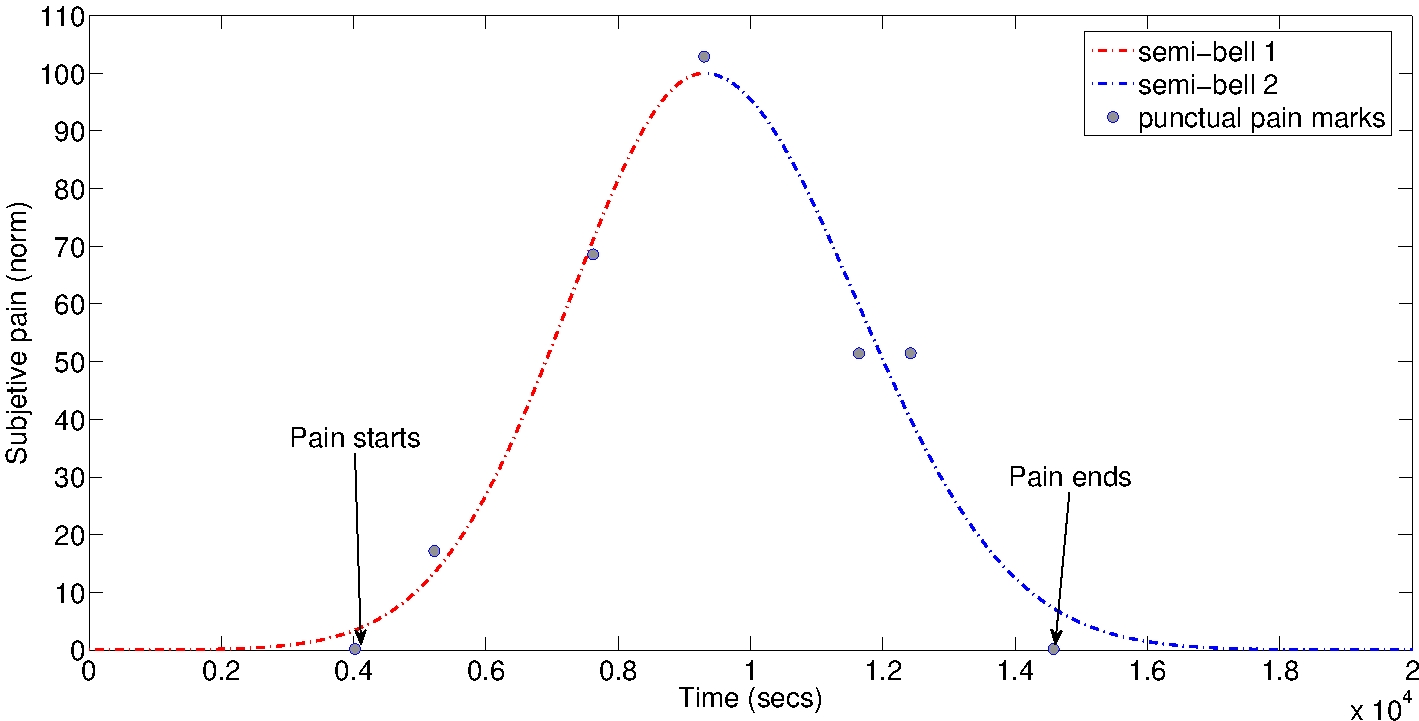
\includegraphics[width=\textwidth]{images/paincurvereal}
\caption{Modeling of subjective pain evolution curve}
\label{fig:paincurve}
\end{figure}

Nevertheless, the target signal we used in our algorithms differs slightly of the curve described: we set the timestamp of the beginning of the aura phase as the first referent point instead of taking the beginning of pain for it. Doing this, we model other specific symptoms of the migraine disease and allow the algorithms to predict earlier the pain.

